\documentclass[11pt,a4paper]{article}
\usepackage[utf8]{inputenc}
\usepackage[T1]{fontenc}
\usepackage[brazilian]{babel}
\usepackage{lmodern}
\usepackage{amsmath,amssymb,bm}
\usepackage{graphicx}
\usepackage{booktabs}
\usepackage{float}
\usepackage{xcolor}
\usepackage{listings}
\usepackage[margin=2.3cm]{geometry}
\usepackage{hyperref}
\usepackage{caption}
\usepackage{subcaption}

\graphicspath{{figuras/}}
\hypersetup{colorlinks=true,linkcolor=blue!50!black,citecolor=blue!50!black,urlcolor=blue!50!black}

\lstset{
  basicstyle=\ttfamily\scriptsize, breaklines=true, columns=fullflexible,
  frame=single, framerule=0.3pt, rulecolor=\color{gray!60},
  backgroundcolor=\color{gray!5}, keepspaces=true, showstringspaces=false,
  commentstyle=\color{green!40!black}, keywordstyle=\color{blue!60!black},
  inputencoding=utf8, extendedchars=true,
  literate={λ}{{$\lambda$}}1 {σ}{{$\sigma$}}1 {δ}{{$\delta$}}1 {×}{{$\times$}}1
           {ã}{{\~a}}1 {á}{{\'a}}1 {â}{{\^a}}1 {é}{{\'e}}1 {ê}{{\^e}}1 {í}{{\'i}}1
           {ó}{{\'o}}1 {ú}{{\'u}}1 {ç}{{\c{c}}}1
}

\newcommand{\E}{\mathbb{E}}
\newcommand{\Var}{\mathrm{Var}}
\newcommand{\bx}{\bm{x}}
\newcommand{\bxi}{\bm{\xi}}

\title{Elementos finitos estocásticos:\\
Karhunen--Loève (analítico, Nyström e Galerkin), Monte Carlo e FORM\\[2mm]
\large Reprodução dos exemplos bidimensionais de Ghanem \& Spanos (2003), Seção 5.3}
\author{Notas de estudo}
\date{16 de novembro de 2026}

\begin{document}
\maketitle
\tableofcontents
\newpage

%=====================================================================
\section{Objetivo e roteiro}
%=====================================================================
Estas notas reúnem, em ordem, o que foi construído e discutido:
\begin{enumerate}
  \item um código de elementos finitos (MEF) para elasticidade plana em \emph{Mathematica}, verificado contra a solução exata (Seção~\ref{sec:det});
  \item a representação do módulo de elasticidade $E(\bx)$ como um \emph{campo aleatório} pela expansão de Karhunen--Loève (KL), resolvida de três maneiras: analítica, Nyström e Galerkin (Seção~\ref{sec:kl});
  \item a placa quadrada do livro (pág.~144--153), com Monte Carlo, e a explicação da diferença aparente para a Fig.~5.46 (Seção~\ref{sec:quadrada});
  \item a análise de confiabilidade: função de estado limite, probabilidade de falha por Monte Carlo e por FORM (Seção~\ref{sec:conf});
  \item o que são as variáveis aleatórias do FORM quando a incerteza é um campo (Seção~\ref{sec:variaveis});
  \item a placa curva do livro (pág.~145, 155 e 168--175), em que o KL analítico não é exato, e a pergunta: \emph{o KL analítico do quadrado serve para a placa curva?} (Seção~\ref{sec:curva}).
\end{enumerate}
Os códigos completos estão na pasta \texttt{codigos/} e reproduzidos no Apêndice.

%=====================================================================
\section{Problema determinístico}\label{sec:det}
%=====================================================================
\subsection{Formulação}
Elasticidade linear em estado plano, $\nu=0$ (com $\nu=0$ os estados planos de tensão e de deformação coincidem).
Com funções de forma $N_a$ e deslocamentos nodais $\bm{u}^e$, a deformação é $\bm{\varepsilon}=\bm{B}\bm{u}^e$ e
\begin{equation}
  \bm{K}^e=\int_{\Omega^e}\bm{B}^{T}\bm{D}\,\bm{B}\,d\Omega
  \approx\sum_{g}\bm{B}_g^{T}\bm{D}\,\bm{B}_g\,w_g\,|\bm{J}_g| ,
  \qquad \bm{K}=\mathop{\mathsf{A}}_{e}\bm{K}^e .
\end{equation}
No código, os graus de liberdade são intercalados por nó $(u_{x1},u_{y1},u_{x2},\dots)$, como na função \texttt{ComputeBN}, e o vetor de deformações tem 6 componentes $(\varepsilon_{xx},\gamma_{xy},\gamma_{xz},\varepsilon_{yy},\gamma_{yz},\varepsilon_{zz})$, com a matriz constitutiva \texttt{Cep} escrita em termos de $\lambda$ e $\mu$ de Lamé.

As funções que faltavam no código original eram: \texttt{MeshInfo}, \texttt{ElementDofs}, \texttt{CalcStiff} (soma nos pontos de Gauss), \texttt{GlobalMatrix} (soma as contribuições repetidas com \texttt{Merge[\dots, Total]}), \texttt{GlobalVector} e \texttt{TopLoad} (carga distribuída consistente: cada aresta de comprimento $L$ recebe $qL/2$ em cada nó).

\subsection{Verificação}
Bloco $[-0{,}5;0{,}5]^2$, base engastada, carga distribuída unitária no topo, $E=1$, $\nu=0$. Como não há efeito de Poisson, o engaste não restringe nada e a solução exata é uniaxial:
\begin{equation}
  \sigma_{yy}=-1,\qquad u_y=-(y+0{,}5),\qquad u_x=0 .
\end{equation}
O elemento bilinear reproduz um campo linear exatamente: o erro máximo em $u_y$ foi $6{,}7\times10^{-16}$ e $|u_x|\le5\times10^{-16}$ (Fig.~\ref{fig:campos}). A malha gerada por \texttt{ToElementMesh[FullRegion[2],\dots,MaxCellMeasure->0.1]} é uma grade $4\times4$ de quadriláteros (\texttt{QuadElement}), igual à do livro.

\begin{figure}[H]
  \centering
  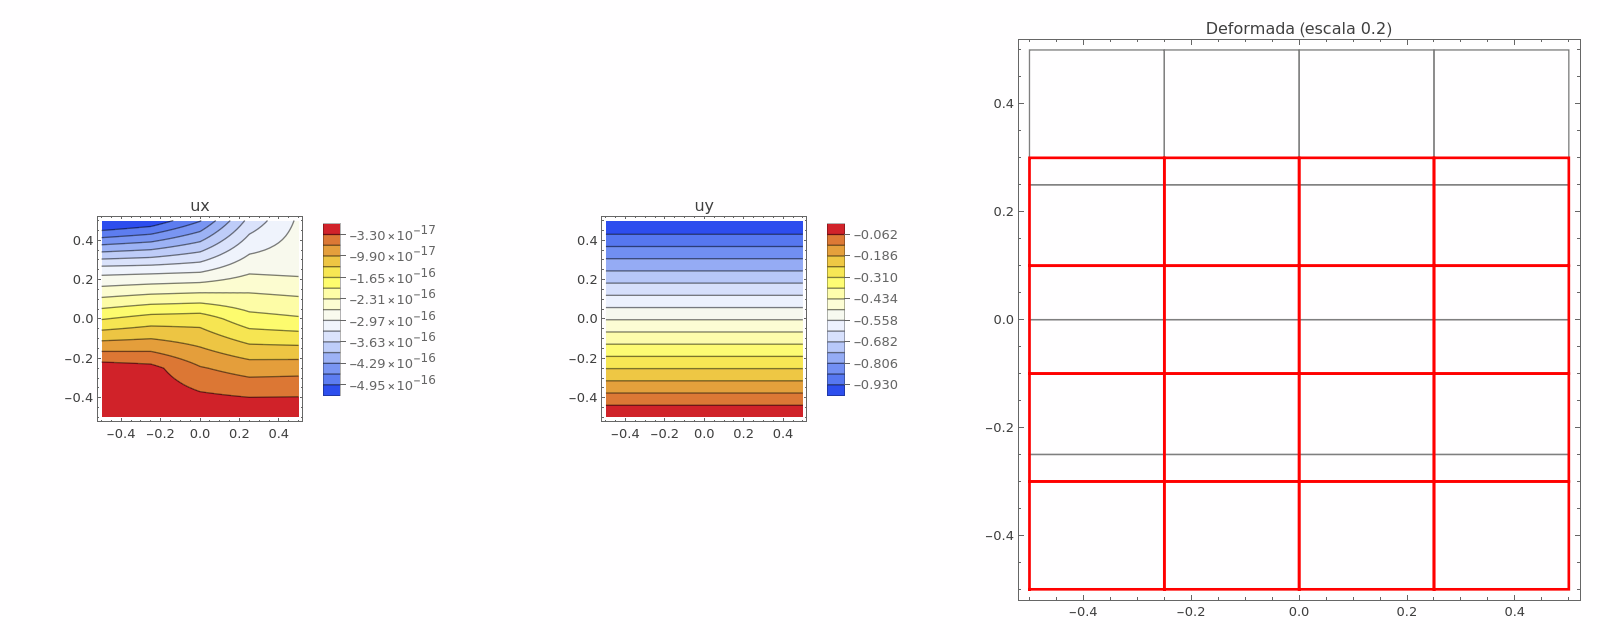
\includegraphics[width=\textwidth]{campos.png}
  \caption{Campos $u_x$ (ruído numérico de $10^{-16}$), $u_y$ e malha deformada (escala 0,2).}
  \label{fig:campos}
\end{figure}

%=====================================================================
\section{Campos aleatórios e a expansão de Karhunen--Loève}\label{sec:kl}
%=====================================================================
\subsection{O campo}
O módulo de elasticidade é um campo gaussiano com média $\langle E\rangle=1$, desvio $\sigma_E$ e covariância exponencial
\begin{equation}
  \mathrm{Cov}[E(\bx),E(\bx')]=\sigma_E^2\,C(\bx,\bx'),\qquad
  C(\bx,\bx')=e^{-|x_1-x_1'|/b_1-|x_2-x_2'|/b_2},
\end{equation}
com comprimentos de correlação $b_1=b_2=1$ (eq.~5.49 do livro).

\subsection{Expansão KL}
O KL escreve o campo como uma soma de formas determinísticas multiplicadas por variáveis aleatórias independentes:
\begin{equation}\label{eq:kl}
  \boxed{E(\bx,\theta)=\langle E\rangle+\sigma_E\sum_{k=1}^{M}\sqrt{\lambda_k}\,f_k(\bx)\,\xi_k(\theta),\qquad \xi_k\sim N(0,1)\ \text{independentes}}
\end{equation}
em que $(\lambda_k,f_k)$ são os autopares da equação integral de Fredholm
\begin{equation}\label{eq:fredholm}
  \int_{\Omega}C(\bx,\bx')\,f_k(\bx')\,d\bx'=\lambda_k f_k(\bx),\qquad
  \int_\Omega f_i f_j\,d\bx=\delta_{ij}.
\end{equation}
Duas propriedades importantes:
\begin{itemize}
  \item $\sum_k\lambda_k=\int_\Omega C(\bx,\bx)\,d\bx=|\Omega|$ (a área do domínio);
  \item a variância representada no ponto $\bx$ é $\sum_{k=1}^{M}\lambda_k f_k(\bx)^2\to1$ quando $M\to\infty$.
\end{itemize}
Ordenando $\lambda_1\ge\lambda_2\ge\dots$, o truncamento em $M$ termos é o \emph{ótimo} no sentido do erro quadrático médio: nenhuma outra base de $M$ funções representa tanta variância \emph{no domínio $\Omega$}.

\subsection{Solução analítica (domínio retangular)}
Para o kernel exponencial separável num retângulo $[-a_1,a_1]\times[-a_2,a_2]$, $f_n(x_1,x_2)=f^{(1)}_i(x_1)f^{(2)}_j(x_2)$ e $\lambda_n=\lambda^{(1)}_i\lambda^{(2)}_j$ (eq.~5.50--5.51). Em cada direção, com $c=1/b$ (eq.~5.56--5.59):
\begin{align}
  &\lambda_i=\frac{2c}{\omega_i^2+c^2},\\
  &i\ \text{ímpar}:\quad c-\omega_i\tan(\omega_i a)=0,\qquad f_i(x)=\frac{\cos(\omega_i x)}{\sqrt{a+\frac{\sin(2\omega_i a)}{2\omega_i}}},\\
  &i\ \text{par}:\quad \omega_i+c\tan(\omega_i a)=0,\qquad f_i(x)=\frac{\sin(\omega_i x)}{\sqrt{a-\frac{\sin(2\omega_i a)}{2\omega_i}}}.
\end{align}
A $i$-ésima raiz está no intervalo $\big((i-1)\tfrac{\pi}{2a},\,i\tfrac{\pi}{2a}\big)$, o que dá um bom chute para o \texttt{FindRoot}. Para $a=0{,}5$, $c=1$: $\omega_1=1{,}3065$ e $\lambda^{(1)}_1=0{,}7388$. Conferência numérica: $\int_{-a}^{a}e^{-c|0{,}2-y|}f_1(y)\,dy\,/\,(\lambda_1 f_1(0{,}2))=1{,}000000$.

Quando $c_1=c_2$, os pares $(i,j)$ e $(j,i)$ têm o mesmo autovalor (modos \emph{degenerados}); por isso $\lambda_2=\lambda_3$, $\lambda_4=\lambda_5$, etc.

\subsection{Método de Nyström}
Substitui a integral de \eqref{eq:fredholm} por uma quadratura nos nós da malha, com pesos $w_n$ (área de cada elemento dividida igualmente entre seus nós):
\begin{equation}
  \sum_{m}C(\bx_n,\bx_m)\,w_m\,f_k(\bx_m)=\lambda_k f_k(\bx_n).
\end{equation}
Para ter uma matriz simétrica, define-se $\bm{W}=\mathrm{diag}(w)$ e resolve-se
\begin{equation}
  \bm{K}_N=\bm{W}^{1/2}\bm{C}\,\bm{W}^{1/2},\qquad \bm{K}_N\bm{v}_k=\lambda_k\bm{v}_k,\qquad f_k(\bx_n)=v_{k,n}/\sqrt{w_n}.
\end{equation}
Com isso $\sum_n w_n f_i(\bx_n)f_j(\bx_n)=\delta_{ij}$ exatamente.
Uma propriedade que será importante: \emph{com todos os modos ($M=$ número de nós), o Nyström reproduz exatamente a matriz de covariância nos nós}, pois $\sum_k\lambda_k\bm{f}_k\bm{f}_k^T=\bm{W}^{-1/2}\bm{K}_N\bm{W}^{-1/2}=\bm{C}$.

\subsection{Método de Galerkin (o do livro, eq.~5.61--5.68)}
Interpola-se $f_k(\bx)=\bm{N}(\bx)\bm{d}_k$ com as funções de forma do MEF e exige-se que o resíduo de \eqref{eq:fredholm} seja ortogonal às funções de forma:
\begin{equation}
  \bm{C}_g\bm{d}_k=\lambda_k\bm{B}\bm{d}_k,\qquad
  \bm{C}_g=\iint \bm{N}^T(\bx)\,C(\bx,\bx')\,\bm{N}(\bx')\,d\bx\,d\bx',\qquad
  \bm{B}=\int\bm{N}^T\bm{N}\,d\bx .
\end{equation}
É um problema de autovalor generalizado; a normalização é $\bm{d}_k^T\bm{B}\bm{d}_k=1$. A integral dupla é feita com os pontos de Gauss de todos os elementos.

\subsection{Elementos finitos com $E$ aleatório}
Interpolando $E$ dos nós para os pontos de Gauss, $\bm{K}$ é \emph{linear} nos valores nodais de $E$. Com \eqref{eq:kl}:
\begin{equation}\label{eq:Kxi}
  \bm{K}(\bxi)=\bm{K}^{(0)}+\sigma_E\sum_{k=1}^{M}\xi_k\,\bm{K}^{(k)},
\end{equation}
que é a eq.~5.72 do livro. $\bm{K}^{(0)}$ é a rigidez com $E=1$ e $\bm{K}^{(k)}$ é a rigidez montada com o ``campo'' $E=\sqrt{\lambda_k}f_k(\bx)$. Essas matrizes são montadas \emph{uma única vez}; cada amostra de Monte Carlo custa só um \texttt{LinearSolve}.

%=====================================================================
\section{Placa quadrada (Ghanem \& Spanos, Fig.~5.44)}\label{sec:quadrada}
%=====================================================================
\begin{figure}[H]
  \centering
  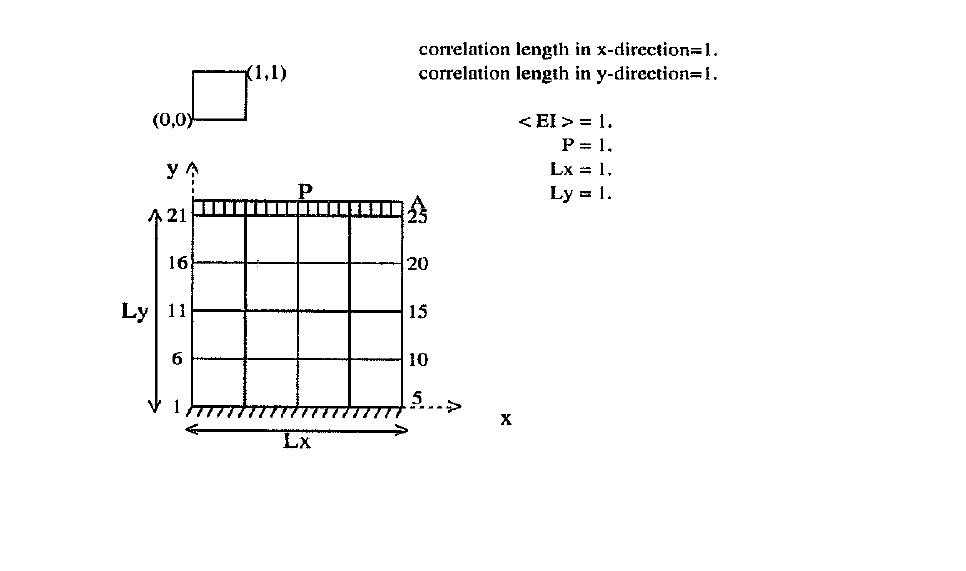
\includegraphics[width=0.55\textwidth]{fig544.png}
  \caption{Problema do livro: placa $1\times1$, malha $4\times4$, base engastada, carga $P=1$ de tração no topo, canto $A$ no topo à direita.}
\end{figure}

\subsection{Autovalores: Nyström $\times$ analítico}
\begin{table}[H]
\centering
\begin{tabular}{lcccccccc}
\toprule
modo & 1 & 2 & 3 & 4 & 5 & 6 & 7 & 8\\
\midrule
Nyström (25 nós) & 0,5446 & 0,1061 & 0,1061 & 0,0403 & 0,0403 & 0,0248 & 0,0248 & 0,0221\\
Analítico        & 0,5458 & 0,1020 & 0,1020 & 0,0333 & 0,0333 & 0,0190 & 0,0158 & 0,0158\\
\bottomrule
\end{tabular}
\caption{Primeiros autovalores. O 1º modo bate em 0,2\%; os modos altos pioram porque 25 pontos de quadratura são poucos para formas oscilantes. Soma dos $\lambda$ do Nyström $=1=|\Omega|$.}
\end{table}

\begin{figure}[H]
  \centering
  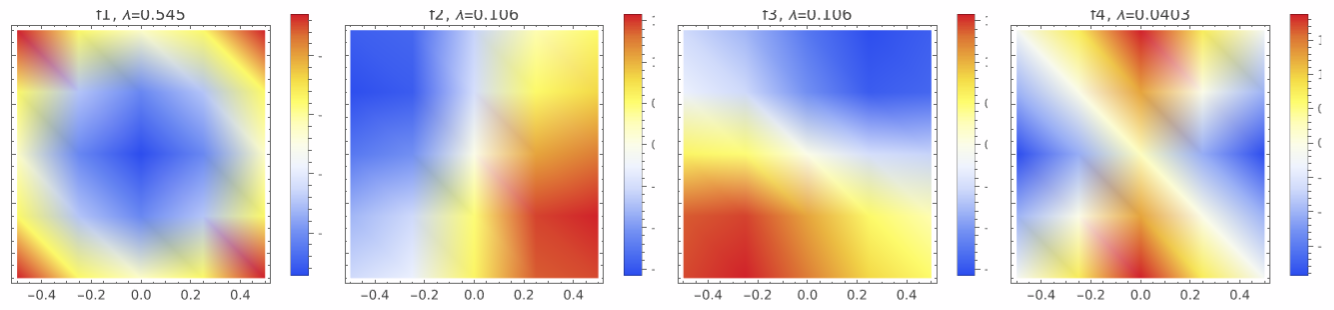
\includegraphics[width=\textwidth]{autofuncoes.png}
  \caption{As quatro primeiras autofunções de Nyström. Os modos 2 e 3 (e 4 e 5) são degenerados.}
\end{figure}

\subsection{Desvio padrão do deslocamento no canto $A$}
Monte Carlo com 5000 amostras de $\bxi$ e \eqref{eq:Kxi}. O deslocamento determinístico é $u_y(A)=1$.

\paragraph{A diferença aparente para o livro.}
À primeira vista, os nossos $\sigma_u$ eram cerca de 2,4 vezes menores que os da Fig.~5.46. A explicação está na legenda: ``$\sigma_{\max}=0{,}433$''. O eixo vertical do livro é $\sigma_u/\sigma_{\max}$, isto é, o desvio normalizado pelo valor obtido em $\sigma_E=0{,}30$ (por isso o último ponto vale $\approx 1$). Multiplicando os pontos do livro por 0,433 as curvas coincidem (Tabela~\ref{tab:sigq}, Fig.~\ref{fig:sigq}).

\begin{table}[H]
\centering
\begin{tabular}{cccccc}
\toprule
$\sigma_E$ & Nyström $M=25$ & Analítico $M=25$ & \textbf{Livro $\times$0,433} & Nyström $M=2$ & Analítico $M=2$\\
\midrule
0,10 & 0,089 & 0,088 & \textbf{0,091} & 0,086 & 0,072\\
0,14 & 0,129 & 0,127 & \textbf{0,139} & 0,123 & 0,103\\
0,20 & 0,200 & 0,197 & \textbf{0,208} & 0,188 & 0,155\\
0,24 & 0,266 & 0,260 & \textbf{0,268} & 0,244 & 0,195\\
0,26 & 0,351 & 0,312 & \textbf{0,303} & 0,289 & 0,218\\
0,30 & 0,474 & 0,481 & \textbf{0,429} & instável & 0,275\\
\bottomrule
\end{tabular}
\caption{$\sigma$ de $u_y(A)$ (Monte Carlo, 5000 amostras, mesmas $\bxi$ para todas as bases).}
\label{tab:sigq}
\end{table}

\begin{figure}[H]
  \centering
  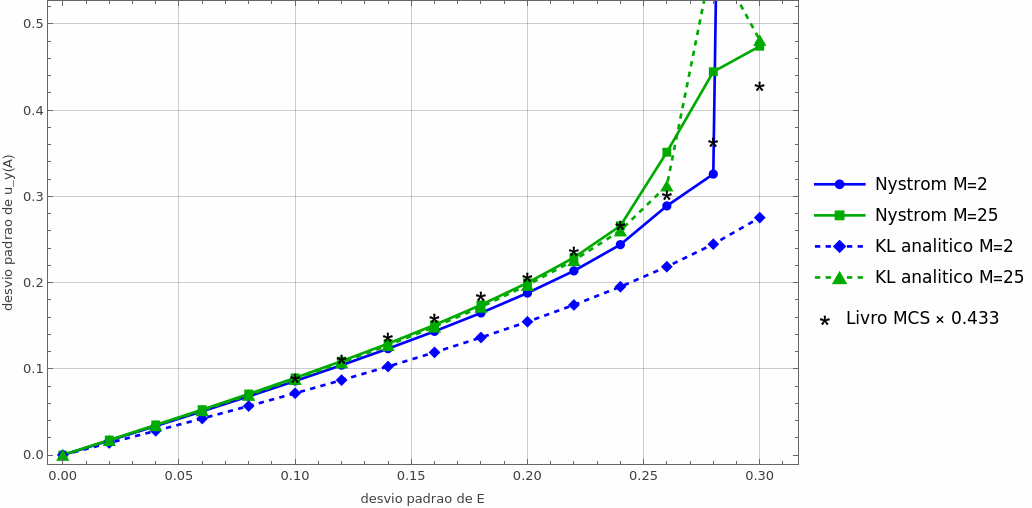
\includegraphics[width=0.8\textwidth]{comparacao2.png}
  \caption{$\sigma$ de $u_y(A)$ em função de $\sigma_E$; pontos do livro já multiplicados por $\sigma_{\max}=0{,}433$.}
  \label{fig:sigq}
\end{figure}

\paragraph{Interpretação.}
\begin{enumerate}
  \item \textbf{Faixa linear.} $\sigma_u\approx0{,}9\,\sigma_E$. Conferência à mão: com $\nu=0$ cada coluna é uma barra em série, $u\approx\int_0^1 dy/E$; em 1ª ordem $\delta u\approx-\int\delta E\,dy$ e
  \[
  \sigma_u\approx\sigma_E\sqrt{\int_0^1\!\!\int_0^1e^{-|y-y'|}dy\,dy'}=\sigma_E\sqrt{2/e}=0{,}858\,\sigma_E .
  \]
  \item \textbf{Subida para $\sigma_E\gtrsim0{,}25$.} O campo gaussiano gera amostras com $E\le0$ em algum nó (26 em 5000 para $\sigma_E=0{,}3$, $M=25$). Como $u\propto1/E$, essas amostras explodem e o desvio passa a depender de poucos casos raros e da semente. O livro tem o mesmo comportamento. Para $\sigma_E$ grande, o modelo fisicamente correto é um campo lognormal.
  \item \textbf{Truncamento.} Com $M=2$ o Nyström quase não perde nada, porque o deslocamento é uma média do campo e é dominado pelo 1º modo. O analítico com $M=2$ perde cerca de 20\%: entre os modos degenerados 2 e 3 ele pega $f_1(x)f_2(y)$, que é ímpar em $y$ e quase não altera $u_y$; o Nyström pega uma combinação ``girada'' dos dois. \emph{Com modos degenerados, qual deles entra no truncamento importa.}
  \item \textbf{Variância representada no canto $A$} (deveria ser 1): Nyström $M=2$: 0,32; $M=4$: 0,55; $M=25$: 1,00. Analítico $M=25$: 0,85.
\end{enumerate}

%=====================================================================
\section{Confiabilidade: Monte Carlo e FORM}\label{sec:conf}
%=====================================================================
\subsection{Função de estado limite}
\begin{equation}
  g(\bxi)=\delta-u_y(A;\bxi),\qquad \text{falha}\iff g\le0,\qquad P_f=P[g\le0].
\end{equation}
No Monte Carlo, uma amostra com $E\le0$ em algum nó também foi contada como falha (com $\sigma_E=0{,}2$ isso não ocorreu).

\subsection{Monte Carlo}
\begin{equation}
  \hat P_f=\frac1N\sum_{s=1}^N\mathbb{1}[g(\bxi_s)\le0],\qquad
  \mathrm{cv}(\hat P_f)=\sqrt{\frac{1-P_f}{N\,P_f}} .
\end{equation}
Para $\mathrm{cv}=10\%$ com $P_f=10^{-3}$ são necessárias cerca de $10^5$ amostras.

\subsection{FORM e o algoritmo HLRF}
O FORM trabalha no espaço normal padrão $\bm{Y}$ e procura o ponto da superfície $g=0$ mais próximo da origem (ponto de projeto $\bm{y}^*$):
\begin{equation}
  \beta=\min\|\bm{y}\|\ \text{ sujeito a }\ g(\bm{y})=0,\qquad P_f\approx\Phi(-\beta).
\end{equation}
A iteração HLRF (Hasofer--Lind--Rackwitz--Fiessler) lineariza $g$ no ponto atual:
\begin{equation}
  \bm{y}^{(k+1)}=\frac{\nabla g^{T}\bm{y}^{(k)}-g(\bm{y}^{(k)})}{\|\nabla g\|^2}\,\nabla g ,
  \qquad \alpha_i^2=\Big(\frac{\partial g/\partial y_i}{\|\nabla g\|}\Big)^2 .
\end{equation}
Os $\alpha_i^2$ (fatores de importância) somam 1 e dizem quanto cada variável pesa na falha.

\paragraph{Gradiente pelo método adjunto.} Com \eqref{eq:Kxi}, derivando $\bm{K}\bm{u}=\bm{F}$:
\begin{equation}
  \frac{\partial\bm{u}}{\partial\xi_k}=-\bm{K}^{-1}\big(\sigma_E\bm{K}^{(k)}\bm{u}\big),\qquad
  \frac{\partial u_A}{\partial\xi_k}=-\sigma_E\,\bm{\lambda}^T\bm{K}^{(k)}\bm{u},\quad \bm{K}\bm{\lambda}=\bm{e}_A .
\end{equation}
O custo é uma fatoração e duas soluções por iteração, para qualquer $M$. Conferido contra diferenças finitas (7 dígitos).

\subsection{Resultados na placa quadrada ($\sigma_E=0{,}2$)}
Iterações do HLRF para $\delta=1{,}4$, Nyström $M=25$: $\beta=2{,}30\to1{,}756\to1{,}672\to1{,}67022\to1{,}670222$ (resíduo $6\times10^{-12}$ na 5ª iteração), $P_f=\Phi(-1{,}670)=0{,}0474$. Fatores de importância: modo 1: 0,70; modo 2: 0,24; modo 3: 0,04; os demais 22 modos: $\approx$2\%.

\begin{table}[H]
\centering
\small
\begin{tabular}{cccccccccc}
\toprule
$\delta$ & $\beta$ (Nys25) & FORM Nys2 & MC Nys2 & FORM Nys25 & MC Nys25 & FORM An2 & MC An2 & FORM An25 & MC An25\\
\midrule
1,2 & 0,97 & 0,158 & 0,157 & 0,167 & 0,176 & 0,116 & 0,120 & 0,164 & 0,170\\
1,3 & 1,34 & 0,082 & 0,083 & 0,089 & 0,097 & 0,049 & 0,051 & 0,087 & 0,090\\
1,4 & 1,67 & 0,042 & 0,043 & 0,047 & 0,053 & 0,020 & 0,022 & 0,046 & 0,049\\
1,5 & 1,95 & 0,022 & 0,022 & 0,025 & 0,028 & 0,0084 & 0,0087 & 0,024 & 0,024\\
1,6 & 2,20 & 0,0116 & 0,0119 & 0,0138 & 0,0161 & 0,0036 & 0,0041 & 0,0129 & 0,0134\\
\bottomrule
\end{tabular}
\caption{$P_f=P[u_y(A)>\delta]$ na placa quadrada; MC com $N=20000$ (cv de 1,5\% a 6\%).}
\label{tab:pfq}
\end{table}

\begin{figure}[H]
  \centering
  \begin{subfigure}{0.49\textwidth}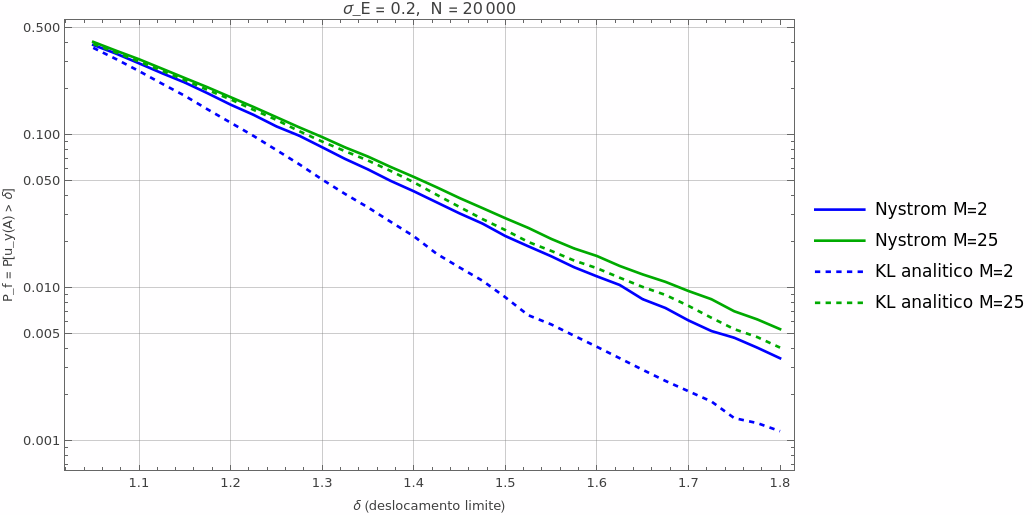
\includegraphics[width=\textwidth]{pf.png}\caption{Monte Carlo, 4 bases.}\end{subfigure}
  \begin{subfigure}{0.49\textwidth}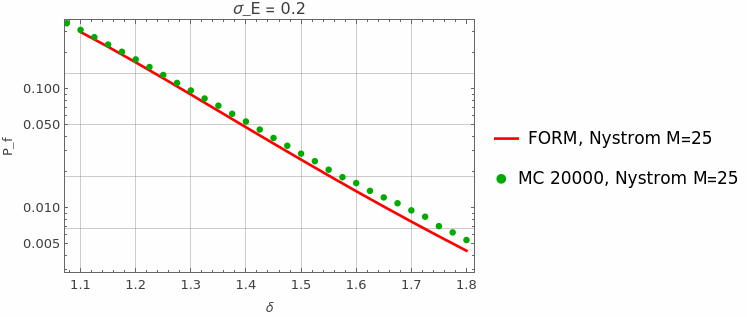
\includegraphics[width=\textwidth]{form.png}\caption{FORM $\times$ MC (Nyström $M=25$).}\end{subfigure}
  \caption{Curvas $P_f(\delta)$ na placa quadrada, $\sigma_E=0{,}2$.}
\end{figure}

\paragraph{Interpretação.}
\begin{enumerate}
  \item Com $M=2$ o FORM coincide com o MC (diferenças dentro do ruído).
  \item Com $M=25$ o FORM fica 5--15\% abaixo do MC. A razão é a curvatura de $g$: $u\propto1/E$ é convexo em $\bxi$, a superfície $g=0$ se curva em direção à origem e cada uma das muitas variáveis ``fracas'' acrescenta um pouco de probabilidade que a linearização ignora. Um SORM corrigiria.
  \item O truncamento pesa \emph{mais} em $P_f$ do que no desvio padrão: o analítico com $M=2$ erra $\sigma_u$ em 20\%, mas $P_f(\delta=1{,}6)$ em 3,5$\times$. A probabilidade de falha depende da cauda.
\end{enumerate}

%=====================================================================
\section{Quais são as variáveis aleatórias do FORM num campo?}\label{sec:variaveis}
%=====================================================================
\subsection{FORM clássico}
No FORM com variáveis $X_1,\dots,X_n$ (por exemplo, duas lognormais de médias 38 e 54), a função \texttt{HLRF} faz
\[
\underbrace{\bm{X}}_{\text{físico}}
\xrightarrow{\ \log\text{ se lognormal}\ }
\underbrace{\bm{Z}}_{\text{normal correlacionado}}
\xrightarrow{\ \bm{L}^{-1}\ }
\underbrace{\bm{Y}}_{\text{normal padrão independente}},
\qquad \bm{Z}=\bm{\mu}+\bm{D}\,\bm{L}\,\bm{Y},
\]
com $\bm{L}$ o fator de Cholesky da matriz de correlação.

\subsection{Campo: duas formas equivalentes}
Um campo é, a rigor, uma variável aleatória em cada ponto. Para usar o FORM é preciso um número finito delas:

\textbf{Forma 1 --- valores nodais.} $X_n=E(\bx_n)$, $n=1,\dots,25$, com \texttt{tipos = "NORMAL"}, \texttt{medias = 1}, \texttt{desvios} $=\sigma_E$ e \texttt{corr = CMAT} (o kernel avaliado entre os nós). Nada muda no FORM, só o número de variáveis e a matriz de correlação deixa de ser diagonal.

\textbf{Forma 2 --- coeficientes do KL.} $X_k=\xi_k$, $k=1,\dots,M$. Comparando \eqref{eq:kl} com $\bm{Z}=\bm{\mu}+\bm{D}\bm{L}\bm{Y}$:
\begin{center}
\begin{tabular}{ll}
\toprule
HLRF & KL\\
\midrule
$\bm{Y}$ (normal padrão independente) & $\bxi$\\
$\bm{L}$ (Cholesky: $\bm{C}=\bm{L}\bm{L}^T$) & $[\sqrt{\lambda_k}f_k(\bx_n)]$ (autovetores: $\bm{C}=(\bm\Phi\sqrt{\bm\Lambda})(\bm\Phi\sqrt{\bm\Lambda})^T$)\\
\bottomrule
\end{tabular}
\end{center}
\emph{O KL é outra fatoração da matriz de correlação.} Por isso, na chamada da \texttt{HLRF} com os $\xi$, usa-se \texttt{medias = 0}, \texttt{Diag = I}, \texttt{L = I}: o KL já fez o papel do $\bm{L}$.

\textbf{Verificação numérica} ($\delta=1{,}4$, $\sigma_E=0{,}2$): forma 1 (25 valores nodais + Cholesky) $\Rightarrow\beta=1{,}670222064$; forma 2 (Nyström, $M=25$) $\Rightarrow\beta=1{,}670222064$. Idênticos.

\subsection{$M$ é o número de variáveis aleatórias --- e não o número de nós}
Com $M=2$ continuam existindo 25 valores de $E$, um por nó, mas todos calculados a partir de 2 números aleatórios:
\[
\underbrace{\begin{bmatrix}E_1\\ \vdots\\ E_{25}\end{bmatrix}}_{25\ \text{valores}}
=1+\sigma_E
\underbrace{\begin{bmatrix}f_1(\bx_1)&f_2(\bx_1)\\ \vdots&\vdots\\ f_1(\bx_{25})&f_2(\bx_{25})\end{bmatrix}}_{25\times2,\ \text{fixa}}
\underbrace{\begin{bmatrix}\sqrt{\lambda_1}\,\xi_1\\ \sqrt{\lambda_2}\,\xi_2\end{bmatrix}}_{2\ \text{aleatórios}} .
\]
Cada modo $f_k$ é uma forma sobre a placa \emph{inteira}; $\xi_k$ diz quanto dessa forma entra na realização. Truncar é ficar com as formas que mais carregam variância (como numa série de Fourier ou numa PCA). Funciona bem quando o comprimento de correlação é grande frente ao domínio (campo suave, $\lambda_k$ decai rápido); com correlação curta são necessários muitos modos.

\subsection{Campo lognormal}
Basta \texttt{tipos = "LOGNORMAL"} na forma nodal; a correlação passa a valer para $\log E$. Resultado ($\delta=1{,}4$, $\sigma_E=0{,}2$): $\beta=1{,}856$, $P_f=0{,}032$ (contra 0,047 no gaussiano): sem a possibilidade de $E\le0$, a cauda de deslocamentos grandes é mais leve.

%=====================================================================
\section{Placa curva (Ghanem \& Spanos, Fig.~5.45)}\label{sec:curva}
%=====================================================================
\subsection{Problema}
Quadrado $[0;1{,}25]^2$ menos um quarto de círculo de raio 1 centrado em $(1{,}25;0)$. A base ($y=0$, $0\le x\le0{,}25$) é engastada, a força total $P=1$ atua na direção $x$ na borda direita ($x=1{,}25$, $1\le y\le1{,}25$) e o canto $A$ é $(1{,}25;1{,}25)$. Estudou-se o deslocamento longitudinal $u_x(A)$.

\begin{figure}[H]
  \centering
  \begin{subfigure}{0.42\textwidth}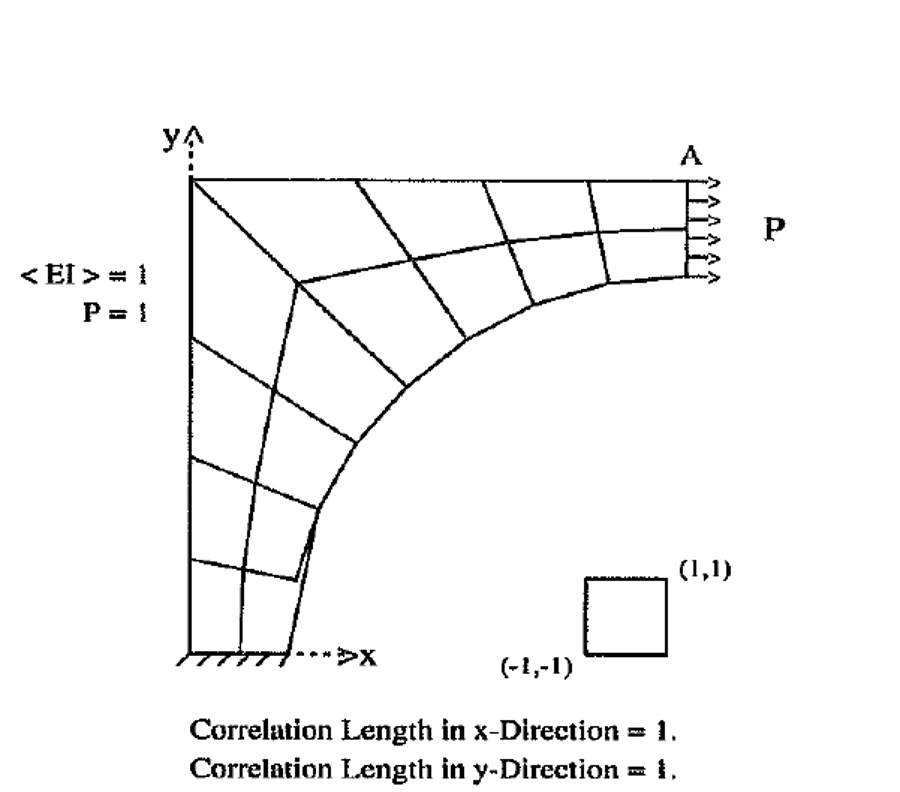
\includegraphics[width=\textwidth]{fig545.png}\caption{Livro, Fig.~5.45.}\end{subfigure}
  \begin{subfigure}{0.56\textwidth}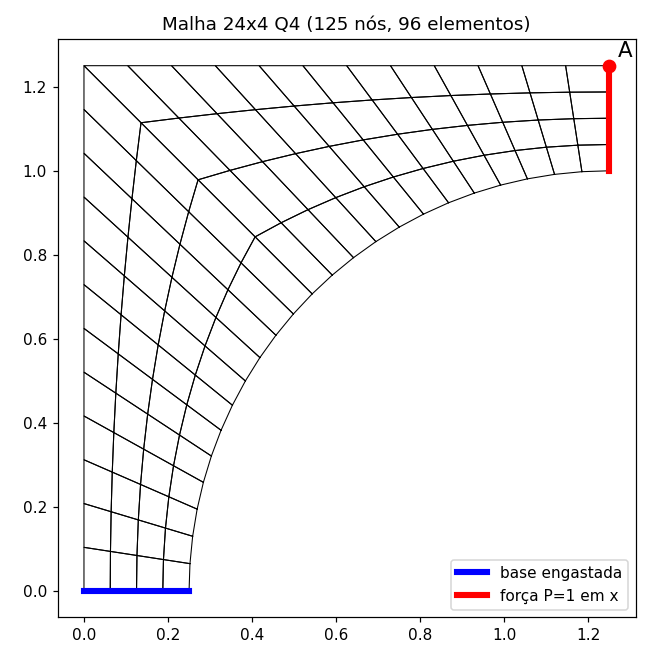
\includegraphics[width=\textwidth]{curva_malha.png}\caption{Malha usada: $24\times4$ Q4 mapeados (125 nós).}\end{subfigure}
  \caption{Placa curva.}
\end{figure}

Implementação em Python (\texttt{codigos/placa\_curva.py}): malha Q4 obtida interpolando entre o arco e o contorno externo em L, $2\times2$ pontos de Gauss, $E=1$, $\nu=0$. Determinístico: $u_x(A)=277{,}8$ (malha $48\times8$: 293,0; a malha de estudo é grosseira, mas serve para comparar as bases entre si). A rigidez foi escrita como $\bm{K}(\bm{E})=\sum_n E_n\bm{G}_n$, com $\bm{G}_n$ a rigidez da ``função chapéu'' do nó $n$, o que serve para as três bases e para o gradiente adjunto ($\partial u_A/\partial E_n=-\bm{\lambda}^T\bm{G}_n\bm{u}$).

\subsection{Três bases KL}
O domínio não é retangular, então a solução analítica não vale diretamente. Foram comparadas:
\begin{itemize}
  \item \textbf{Nyström} na placa;
  \item \textbf{Galerkin} na placa (o método do livro para a placa curva);
  \item \textbf{KL analítico do quadrado envolvente} $[0;1{,}25]^2$ ($a=0{,}625$), avaliado nos nós da placa.
\end{itemize}

\paragraph{Por que o KL do quadrado pode servir?} O campo definido no quadrado, restrito à placa, tem \emph{exatamente} a covariância correta na placa (o kernel só depende de $\bx-\bx'$). Os $\xi_k$ continuam independentes. Então a representação é \emph{válida} e converge quando $M\to\infty$. O que se perde é a \emph{otimalidade}: as funções $f_k$ são ortonormais no quadrado, não na placa, e parte da ``variância'' de cada modo é gasta na região do quadrado que não pertence à placa.

\begin{table}[H]
\centering
\begin{tabular}{lcccccccc}
\toprule
modo & 1 & 2 & 3 & 4 & 5 & 6 & 7 & 8\\
\midrule
Nyström   & 0,411 & 0,116 & 0,050 & 0,035 & 0,024 & 0,017 & 0,014 & 0,010\\
Galerkin  & 0,414 & 0,116 & 0,050 & 0,034 & 0,024 & 0,017 & 0,013 & 0,010\\
Quadrado  & 0,746 & 0,170 & 0,170 & 0,059 & 0,059 & 0,039 & 0,028 & 0,028\\
\bottomrule
\end{tabular}
\caption{Autovalores. Nyström e Galerkin concordam (soma $\approx$ área da placa, 0,778). Os do quadrado somam a área do quadrado (1,562) e \emph{não} são autovalores da placa. Na placa não há mais degenerescência (a simetria do quadrado foi quebrada).}
\end{table}

\paragraph{Ortogonalidade na placa.} $\max_{i,j\le6}\big|\int_{\text{placa}}f_if_j-\delta_{ij}\big|$: Nyström 0,000; Galerkin 0,13 (efeito da quadratura nodal usada para medir); quadrado \textbf{0,53}. As funções do quadrado não são ortogonais na placa.

\begin{figure}[H]
  \centering
  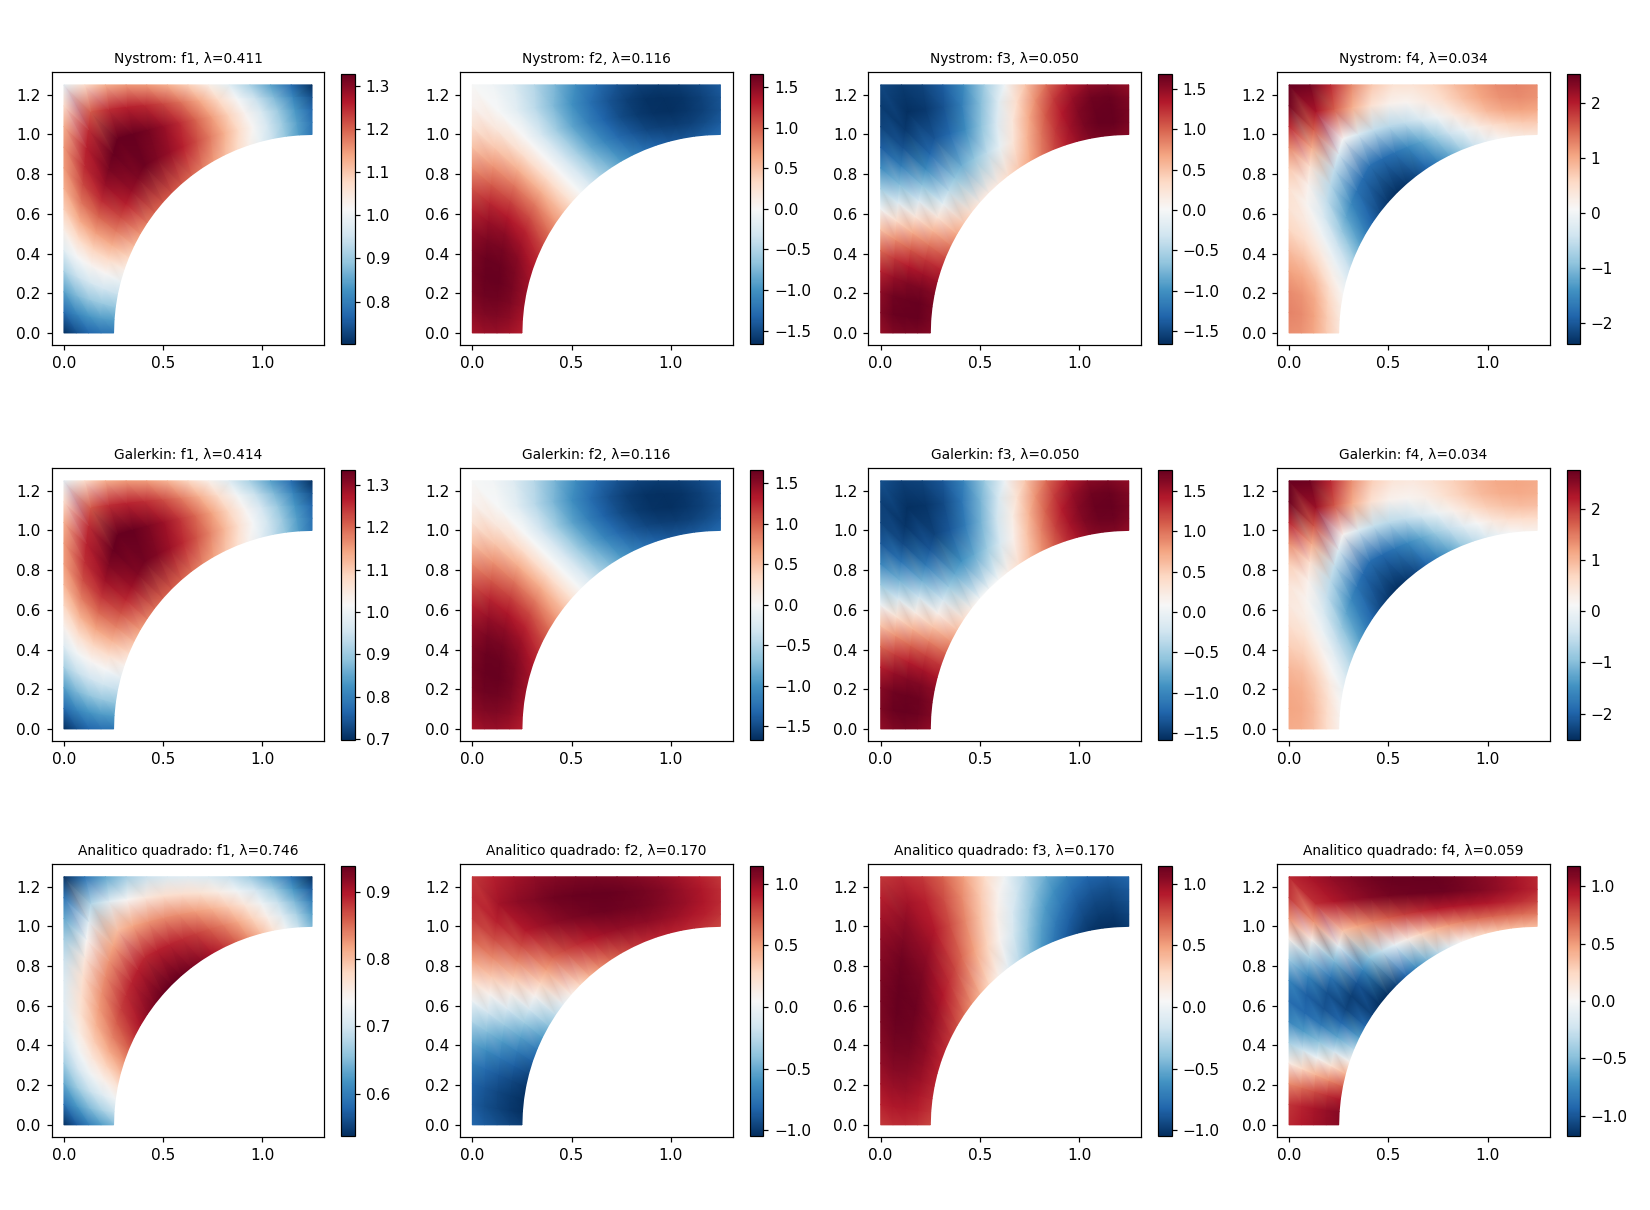
\includegraphics[width=\textwidth]{curva_modos.png}
  \caption{Quatro primeiras autofunções de cada base. Nyström e Galerkin são praticamente iguais; as do quadrado são as do quadrado ``recortadas''.}
\end{figure}

\subsection{Qualidade da representação do campo}
\begin{table}[H]
\centering
\begin{tabular}{rccccccccc}
\toprule
 & \multicolumn{3}{c}{Nyström} & \multicolumn{3}{c}{Galerkin} & \multicolumn{3}{c}{Quadrado}\\
\cmidrule(lr){2-4}\cmidrule(lr){5-7}\cmidrule(lr){8-10}
$M$ & $\bar v$ & $v_A$ & $e_C$ & $\bar v$ & $v_A$ & $e_C$ & $\bar v$ & $v_A$ & $e_C$\\
\midrule
2   & 0,68 & 0,42 & 0,199 & 0,68 & 0,42 & 0,200 & 0,57 & 0,33 & 0,303\\
4   & 0,79 & 0,59 & 0,110 & 0,80 & 0,59 & 0,111 & 0,72 & 0,49 & 0,146\\
6   & 0,84 & 0,69 & 0,071 & 0,86 & 0,69 & 0,072 & 0,79 & 0,60 & 0,091\\
10  & 0,89 & 0,79 & 0,041 & 0,92 & 0,80 & 0,044 & 0,84 & 0,67 & 0,059\\
20  & 0,94 & 0,87 & 0,020 & 0,99 & 0,90 & 0,029 & 0,90 & 0,78 & 0,030\\
40  & 0,97 & 0,94 & 0,009 & 1,05 & 1,03 & 0,028 & 0,94 & 0,86 & 0,016\\
125 & 1,00 & 1,00 & 0,000 & 1,09 & 1,10 & 0,029 & 0,97 & 0,94 & 0,007\\
\bottomrule
\end{tabular}
\caption{$\bar v$: variância de $E$ média na placa; $v_A$: variância no canto $A$ (exato: 1); $e_C=\|\bm{C}_M-\bm{C}\|_F/\|\bm{C}\|_F$: erro da covariância nos nós.}
\label{tab:rep}
\end{table}
O KL do quadrado precisa de cerca de \textbf{duas vezes mais modos} para representar o campo tão bem quanto Nyström/Galerkin ($M=10$ do quadrado $\approx$ $M=4$--6 das bases da placa). O Galerkin com muitos modos passa um pouco de 1 em variância: os modos altos não são bem resolvidos por funções de forma lineares numa malha grosseira (a projeção oscila); para os modos que importam ele coincide com o Nyström.

\begin{figure}[H]
  \centering
  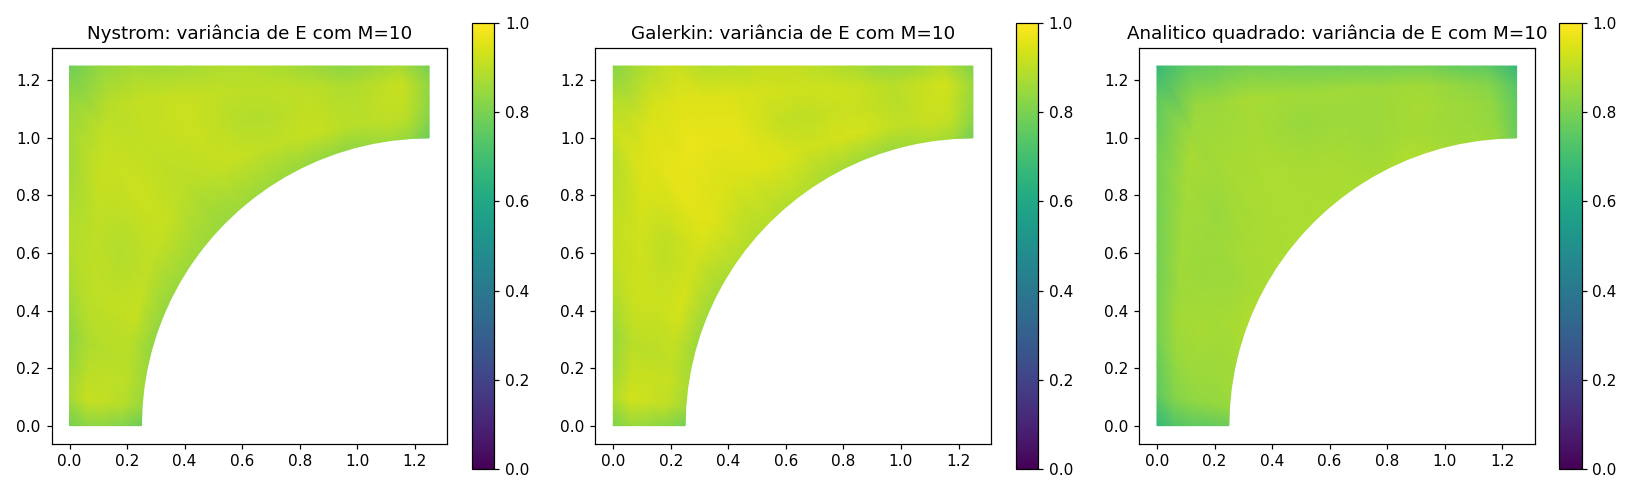
\includegraphics[width=\textwidth]{curva_variancia.png}
  \caption{Variância de $E$ representada com $M=10$. O KL do quadrado deixa a ponta livre (perto de $A$) e a base com menos variância.}
\end{figure}

\subsection{Desvio padrão de $u_x(A)$ e comparação com o livro}
O livro (Fig.~5.66, $M=4$) normaliza por $\sigma_{\max}=19{,}4$. Como o $u_{\det}$ do livro não é dado (depende de como $P$ e a espessura foram definidos), a comparação natural é a da \emph{forma} da curva: no livro $\sigma_u(0{,}20)/\sigma_u(0{,}10)=0{,}475/0{,}215=2{,}21$ e $\sigma_u(0{,}28)/\sigma_u(0{,}10)=3{,}9$; aqui (Nyström $M=4$) obtém-se 2,2 e 3,7.

\begin{table}[H]
\centering
\begin{tabular}{cccccc}
\toprule
$\sigma_E$ & Nyström $M=4$ & Galerkin $M=4$ & Quadrado $M=4$ & Nyström todos & Quadrado todos\\
\midrule
0,04 & 0,033 & 0,033 & 0,031 & 0,034 & 0,034\\
0,08 & 0,066 & 0,067 & 0,063 & 0,069 & 0,068\\
0,12 & 0,102 & 0,103 & 0,096 & 0,107 & 0,105\\
0,16 & 0,141 & 0,142 & 0,132 & 0,149 & 0,146\\
0,20 & 0,185 & 0,186 & 0,172 & 0,199 & 0,194\\
0,24 & 0,239 & 0,239 & 0,220 & 0,266 & 0,256\\
0,28 & 0,311 & 0,309 & 0,283 & 0,423 & 0,420\\
\bottomrule
\end{tabular}
\caption{$\sigma$ de $u_x(A)/u_{\det}$, Monte Carlo com 5000 amostras.}
\end{table}

\begin{figure}[H]
  \centering
  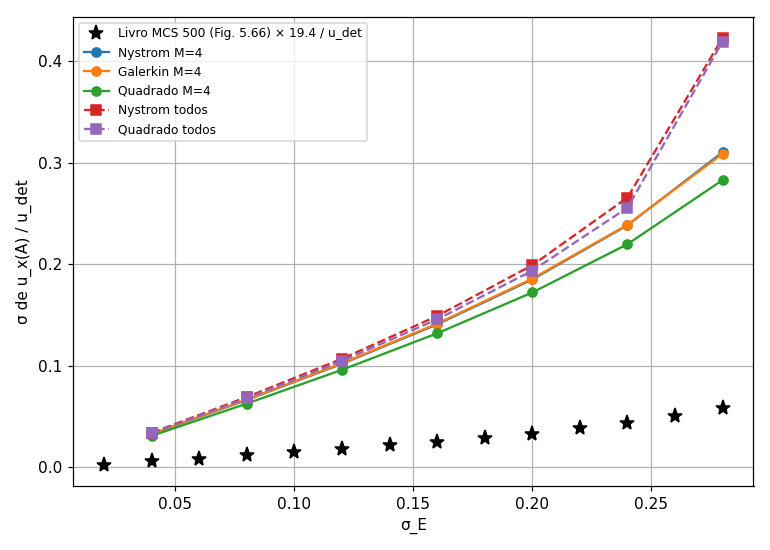
\includegraphics[width=0.75\textwidth]{curva_sigma.png}
  \caption{$\sigma_u/u_{\det}$ na placa curva. Os pontos do livro estão na escala $19{,}4/u_{\det}$ e servem só para comparar a forma (o $u_{\det}$ do livro não é conhecido).}
\end{figure}

\subsection{Probabilidade de falha: FORM $\times$ Monte Carlo}
$g=\delta-u_x(A)$ com $\delta=f\,u_{\det}$, $\sigma_E=0{,}2$, MC com $N=20000$ (as mesmas amostras para todas as bases).
\begin{table}[H]
\centering
\small
\begin{tabular}{lrcccccccc}
\toprule
base & $M$ & FORM 1,3 & MC 1,3 & FORM 1,5 & MC 1,5 & FORM 1,7 & MC 1,7 & $\beta(1{,}5)$ & iter.\\
\midrule
Nyström & 2 & 0,0634 & 0,0677 & 0,0139 & 0,0135 & 0,0033 & 0,0035 & 2,201 & 8\\
Nyström & 4 & 0,0810 & 0,0854 & 0,0218 & 0,0224 & 0,0064 & 0,0067 & 2,017 & 8\\
Nyström & 10 & 0,0883 & 0,0963 & 0,0257 & 0,0271 & 0,0081 & 0,0092 & 1,948 & 10\\
Nyström & 20 & 0,0886 & 0,0985 & 0,0259 & 0,0278 & 0,0082 & 0,0099 & 1,945 & 10\\
Nyström & 125 & 0,0890 & 0,1002 & 0,0261 & 0,0289 & 0,0083 & 0,0100 & 1,941 & 10\\
\midrule
Galerkin & 2 & 0,0637 & 0,0679 & 0,0140 & 0,0136 & 0,0034 & 0,0036 & 2,198 & 8\\
Galerkin & 4 & 0,0816 & 0,0862 & 0,0222 & 0,0232 & 0,0066 & 0,0069 & 2,011 & 8\\
Galerkin & 10 & 0,0891 & 0,0973 & 0,0262 & 0,0288 & 0,0084 & 0,0095 & 1,940 & 10\\
Galerkin & 20 & 0,0897 & 0,0994 & 0,0265 & 0,0303 & 0,0085 & 0,0099 & 1,935 & 10\\
Galerkin & 125 & 0,0901 & 0,1017 & 0,0267 & 0,0308 & 0,0086 & 0,0102 & 1,932 & 10\\
\midrule
Quadrado & 2 & 0,0446 & 0,0459 & 0,0071 & 0,0072 & 0,0013 & 0,0015 & 2,451 & 9\\
Quadrado & 4 & 0,0712 & 0,0718 & 0,0172 & 0,0181 & 0,0045 & 0,0052 & 2,115 & 9\\
Quadrado & 10 & 0,0847 & 0,0902 & 0,0238 & 0,0258 & 0,0073 & 0,0081 & 1,981 & 9\\
Quadrado & 20 & 0,0878 & 0,0964 & 0,0254 & 0,0282 & 0,0080 & 0,0088 & 1,952 & 10\\
Quadrado & 125 & 0,0886 & 0,0981 & 0,0259 & 0,0289 & 0,0082 & 0,0092 & 1,945 & 10\\
\bottomrule
\end{tabular}
\caption{$P_f=P[u_x(A)>f\,u_{\det}]$ na placa curva.}
\label{tab:pfc}
\end{table}

\begin{figure}[H]
  \centering
  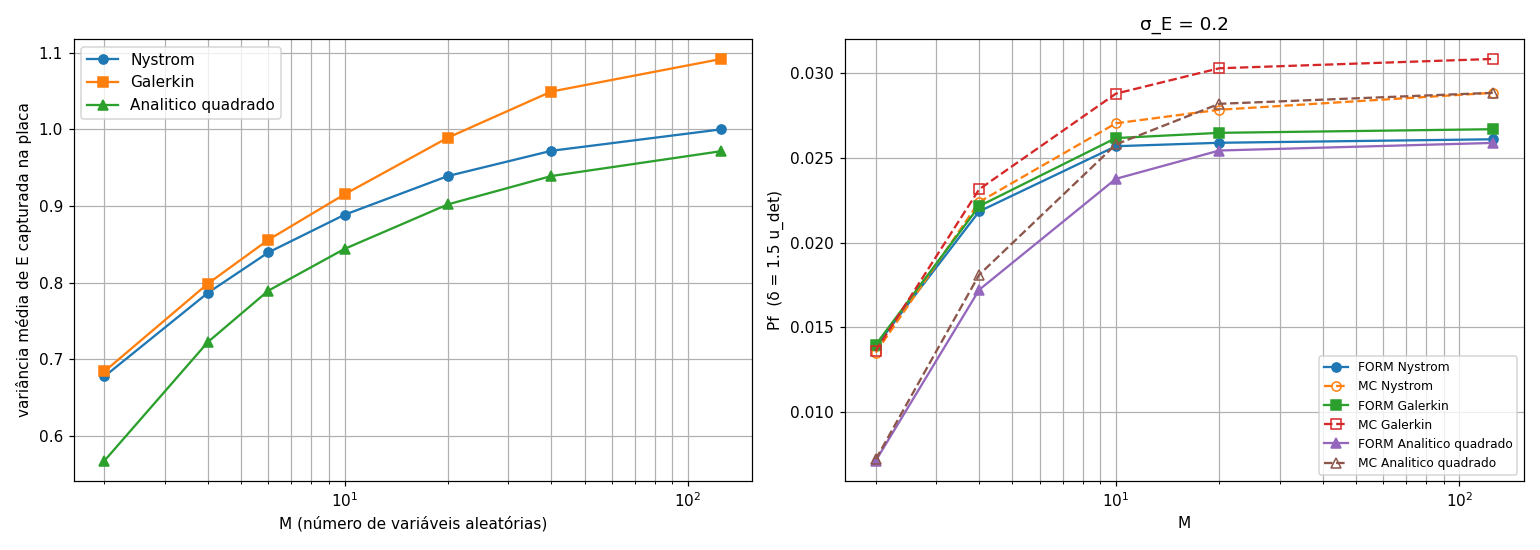
\includegraphics[width=\textwidth]{curva_convergencia.png}
  \caption{Esquerda: variância média capturada em função de $M$. Direita: $P_f$ ($\delta=1{,}5\,u_{\det}$) em função de $M$, FORM (cheio) e MC (vazado).}
\end{figure}

\paragraph{Observações.} Como na placa quadrada, o FORM coincide com o MC para $M$ pequeno e fica 5--15\% abaixo para $M$ grande (curvatura de $g$). Fatores de importância no ponto de projeto ($f=1{,}5$, todos os modos): Nyström $\alpha^2=(0{,}44;\,0{,}33;\,0{,}14;\,0{,}02;\,0{,}04;\dots)$, com 99\% nos 8 primeiros modos; quadrado $\alpha^2=(0{,}47;\,0{,}15;\,0{,}19;\,0{,}02;\,0{,}04;\,0{,}07;\dots)$, 96\% nos 8 primeiros. Na placa curva o 2º e o 3º modos pesam mais do que na quadrada: a falha depende de como $E$ se distribui ao longo do arco (flexão), e não só da média. Nas figuras de convergência, as cores de FORM e MC de uma mesma base não coincidem (ciclo de cores do \texttt{matplotlib}); guie-se pela legenda.

\subsection{O KL analítico serve para a malha curva?}
\begin{enumerate}
  \item \textbf{Serve como representação válida:} restrito à placa, o campo do quadrado tem a covariância correta, e $P_f$ converge para os mesmos valores do Nyström e do Galerkin quando $M$ cresce (Tabela~\ref{tab:pfc}). O erro de covariância com todos os modos é 0,7\%.
  \item \textbf{Mas não é eficiente:} com o mesmo $M$ ele representa menos variância (Tabela~\ref{tab:rep}) e subestima $P_f$. Com $M=2$, $P_f(1{,}5\,u_{\det})$ é cerca de \textbf{metade} do valor das bases da placa (0,0071 contra 0,0139); com $M=4$, cerca de 20\% menor; a diferença só fica pequena com $M\approx20$.
  \item \textbf{Os autovalores do quadrado não são os da placa} e não devem ser usados como tal (por exemplo, para decidir o truncamento pela fração $\sum_{k\le M}\lambda_k/|\Omega|$).
  \item \textbf{Para uso prático}, Nyström e Galerkin na própria malha são baratos (um problema de autovalor do tamanho do número de nós) e dão a base ótima. O KL do quadrado é útil como verificação, ou quando o domínio é quase retangular, ou se for usado com mais modos.
\end{enumerate}

%=====================================================================
\section{Conclusões}
%=====================================================================
\begin{itemize}
  \item O MEF reproduz exatamente a solução uniaxial do problema determinístico.
  \item O método de Nyström (código do usuário) reproduz os autovalores analíticos do KL na placa quadrada (0,2\% no 1º modo) e, com todos os modos, reproduz exatamente a covariância nodal.
  \item Os resultados da placa quadrada coincidem com os do livro, uma vez que se percebe que a Fig.~5.46 está normalizada por $\sigma_{\max}=0{,}433$.
  \item No KL, as variáveis aleatórias são os $M$ coeficientes $\xi_k$; o KL é uma fatoração da covariância equivalente ao Cholesky da forma nodal (mesmo $\beta$ com todos os modos).
  \item O FORM (HLRF com gradiente adjunto) converge em 5--10 iterações e concorda com o MC; com muitas variáveis subestima $P_f$ em 5--15\% por causa da curvatura de $g$.
  \item O truncamento afeta mais $P_f$ do que o desvio padrão; com modos degenerados a escolha do modo importa.
  \item Na placa curva, o KL analítico do quadrado envolvente é uma representação válida mas ineficiente: precisa de cerca do dobro de modos e, com poucos modos, subestima $P_f$.
\end{itemize}

\appendix
\section{Códigos}
\subsection{MEF determinístico e Monte Carlo (Mathematica)}
\lstinputlisting[language=Mathematica,caption={elast.wl --- MEF determinístico}]{codigos/elast.wl}
\lstinputlisting[language=Mathematica,caption={bloco.wl --- Nyström, $\bm{K}^{(k)}$ e Monte Carlo}]{codigos/bloco.wl}
\lstinputlisting[language=Mathematica,caption={bloco2.wl --- KL analítico}]{codigos/bloco2.wl}
\lstinputlisting[language=Mathematica,caption={bloco3.wl --- probabilidade de falha por Monte Carlo}]{codigos/bloco3.wl}
\lstinputlisting[language=Mathematica,caption={hlrf.wl --- algoritmo HLRF}]{codigos/hlrf.wl}
\lstinputlisting[language=Mathematica,caption={bloco4.wl --- FORM com gradiente adjunto}]{codigos/bloco4.wl}
\lstinputlisting[language=Mathematica,caption={bloco5.wl --- FORM com valores nodais (Cholesky) e lognormal}]{codigos/bloco5.wl}
\subsection{Placa curva (Python)}
\lstinputlisting[language=Python,caption={placa\_curva.py}]{codigos/placa_curva.py}

\end{document}
